\documentclass[a4paper,10pt]{article}

\usepackage[utf8]{inputenc}
\usepackage[spanish, activeacute]{babel}
\usepackage{graphicx}
\usepackage{fancybox}
\usepackage[table]{xcolor}

\title{La batalla de Iwo Jima}

\author{Catalano, Juan Ignacio \crcr Palombo, Martín \crcr Pose, Alberto Miguel \crcr Vázquez, Santiago Luis}

\date{}

\begin{document}

\maketitle

\abstract{En el presente artículo se modela un combate guerra-guerra, considerando las fuerzas como medida del poderío de ambas partes y 
analizando el modelo construído para obtener conclusiones mediante su observación. De dicho análisis se desprende que el uso del modelo planteado
resulta adecuado para simular esta batalla, obteniendose resultados similares a los reales. También se analiza el comportamiento del sistema,
mediante la observación del modelo, variando las funciones de refuerzos enviados a la batalla. Además se realiza una deducción analítica que
concluye en una interesante descripción de la relación de efectividad de combate entre ambas fuerzas.}

\newpage

\section{Introducci\'on}

En el presente art\'iculo se explica la realizaci\'on de la simulaci\'on del sistema correspondiente a un combate entre dos fuerzas, 
en particular, rememorando la batalla de Iwo jima, entre los Estados Unidos de Am\'erica y Jap\'on. Para ello, en la primer secci\'on se 
presenta el modelo utilizado para realizar dicha simulaci\'on. En la segunda secci\'on se demuestra un resultado matem\'atico-f\'isico cuya 
consecuencia se explica en la misma secci\'on. En la secci\'on tres se presentan los resultados obtenidos a partir de la simulaci\'on y 
por \'ultimo, en la secci\'on cuatro se agrupan las conclusiones obtenidas durante la realizaci\'on del trabajo.

\section{``La mejor victoria es vencer sin combatir''}
Para modelar este sistema se considerab dos fuerzas ($x^1(t), x^2(t)$) cuya medida representa el poderío de ambas partes del combate. El vector definido como:

\begin{equation}
x(t) = ( x^1(t), x^2(t) )^T \label{eq:state_vector}
\end{equation}

representa el vector de estado, es decir, el poderío de ambas partes en el instante $t$. El espacio de estados se considera como la cantidad de 
unidades de combate, considerando todo tipo de ellas (individuos, equipos, recursos, etc). Como es de esperarse, las entradas al sistema estan 
dadas por los refuerzos enviados por cada uno de los países.\\
Hasta aquí, la representación del modelo de combate. Pero en particular, nos referimos a un combate de tipo guerra-guerra, es decir, convencional.
En este caso, las pérdidas en combate están solamenten dadas por el tamaño de la fuerza contraria, con lo cual nuestro modelo queda descripto de la
siguiente manera:

\begin{equation}
\dot{x}^1(t) = -ax^1(t) - c_{21} x^2(t)\end{equation}
\begin{equation}
\dot{x}^2(t) = -bx^2(t) - c_{12} x^1(t)\end{equation}

Siendo $a$ y $b$ constantes positivas que representan las tasas unitarias de pérdidas operativas y $c_{12}, c_{21}$ tambien constantes positivas
que representan las tasas de efectividad de ataque de la fuerza 1 sobre la 2 y de la fuerza 2 sobre la 1 respectivamente.

\section{Recordando la historia}

En esta sección se utiliza una adaptación del modelo presentado anteriormente para simular el sistema dado por el combate entre Japón y 
Estados Unidos de América, en la ciudad de Iwo Jima en febrero de 1945. Inicialmente Japón cuenta con una fuerza de 21500 unidades 
atrincheradas en el lugar, mientras que su enemigo incialmente no dispone de unidades en Iwo Jima y envía refuerzos siguiendo el siguiente 
régimen:

\begin{equation}
f(t) = \left\{ 
    \begin{array}{l l}
    54000 & \quad 0 \leq t < 1 \\
    0 & \quad 1 \leq t < 2\\
    6000 & \quad 2 \leq t < 3\\
    0 & \quad 3 \leq t < 5\\
    13000 & \quad 5 \leq t < 6\\
    0 & \quad t \leq 6\\
    \end{array} \right.
\end{equation}
Siendo $f$ la función que describe la llegada de refuerzos de los Estados Unidos. Como se considera que Japón no envía refuerzos durante este
combate, el modelo resulta descripto por:

\begin{equation}
 \dot{x}^1 = -\alpha x^2 + f(t)
\end{equation}

\begin{equation}
\dot{x}^2 = -\beta x^1
\end{equation}

\section{Poder K}

El primer resultado obtenido, es meramente analítico y es presentado en esta sección. A partir de una demostración matemática
obtenemos una relación entre las fuerzas de combate y una constante (constante de integración) que determina y controla dicho nexo. 
A continuación se presenta la deducción realizada y luego se detallan las conclusiones obtenidas.

Tenemos

\begin{eqnarray}
\dot{x} & = & -\alpha y\label{eq:ydot}\\
\dot{y} & = & -\beta x\end{eqnarray}


Despejando, obtenemos la expresión

\begin{equation}
\frac{\partial x}{\partial t}=-\alpha y\end{equation}


Como sabemos que $\frac{\partial x}{\partial t}=\frac{\partial x}{\partial y}\frac{\partial y}{\partial t}$:

\begin{equation}
\frac{\partial x}{\partial y}\dot{y}=\frac{\partial x}{\partial y}\frac{\partial y}{\partial t}=-\alpha y\end{equation}


Reemplazando con la ecuación \ref{eq:ydot} resulta

\begin{equation}
-\frac{\partial x}{\partial y}\beta x=-\alpha y\end{equation}


Reemplazando adecuadamente los diferenciales tenemos 

\begin{equation}
-\beta\intop x\partial x=-\alpha\int y\partial y\end{equation}


De lo cual obtenemos

\begin{equation}
\alpha\frac{y^{2}}{2}-\beta\frac{x^{2}}{2}=k\end{equation}


Que tomando $K=2k$ se puede reescribir de la siguiente manera:

\begin{equation}
\alpha y^{2}-\beta x^{2}=K\label{eq:obtenida}\end{equation}


Como se puede observar claramente, se obtiene una relación entre ambas fuerzas de combate, regida por una constante a la cual denominamos $K$. 
Esta constante resulta muy interesante para analizar. Es por ello que analizamos los tres casos de posibles rangos de valores de $K$, explicando
su resultado en el comportamiento del sistema.
\begin{itemize}
\item Si $K>0$ la fuerza descripta por $y$ resulta claramente mayor a la descripta por $x$, resultando en una inclincación hacia la victoria
del primero.
\item Si $K<0$ ocurre lo opuesto a lo descritpo en el punto anterior.
\item El caso que encontramos más interesante es cuando $K=0$. En este caso, la relación entre ambas fuerzas describe una recta, que determina
el grado de efectividad de las unidades militares de una fuerza sobre la otra. Es decir, una vez fijada la pendiente, se puede establecer que
cantidad de unidades son necesarias de una fuerza, ante la presencia de determinada cantidad de unidades enemigas. Esto puede servir también
para calcular y analizar estadísticas de efectividad de las unidades en combate contra determinado contrincante.
\end{itemize}



\section{Reviviendo la historia}

En esta sección se presentan los resultados obtenidos al realizar la simulación del combate. Por un lado, se ejecutó la simulación para obtener las 
trayectorias correspondientes a ambas fuerzas. En la gráfica presentada en la Figura \ref{fig:trays} se pueden ver ambas trayectorias. 
De este podemos observar como, si bien inicialmente las fuerzas militares del Japón eran ampliamente superiores, el hecho de no disponer de 
refuerzos, como en el caso estadounidense, llevó a una rápida extinción del poderío militar presente en la zona. Por parte de los 
Estados Unidos, se vé como si bien su fuerza fue decreyendo a un ritmo similar a la japonesa, la mayor presencia militar llevó a que finalmente
se note una clara preponderancia de este país en el conflicto. También podemos observar un decaimiento lineal en el caso de las fuerzas japonesas,
en contraparte con uno más exponencial (aunque bastante suavizado) por parte de las estadounidenses.\\
Por otro lado, realizamos la gráfica mostrada en la Figura \ref{fig:realvssim} en la cual se presentan los resultados reales de la batalla 
(presentados para la fuerza estadounidense),superpuesto con los resultados arrojados por la simulación. Aquí podemos observar que la función
descripta por la simulación aproxima de manera bastante precisa los resultados reales. Podemos observar el desembarco, en la primer etapa, 
donde vemos claramente como aumenta rápidamente la cantidad de unidades. A su vez, durante los primeros 5 días al recibirse los refuerzos, se
puede ver como se producen picos, donde los aumentos estan dados por la llegada de nuevas unidades y las disminuciones más bruscas estan dadas
por las bajas producidas durante el asentamiento de las tropas en el área de batalla.

\begin{figure}[h]
\begin{center}
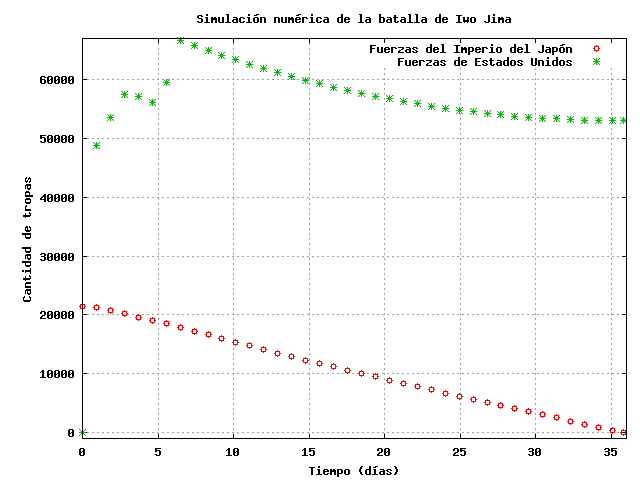
\includegraphics[width=12cm]{jap_vs_usa.png}
\caption{\label{fig:trays}Resultados del combate simulado.}
\end{center}
\end{figure}

\begin{figure}[h]
\begin{center}
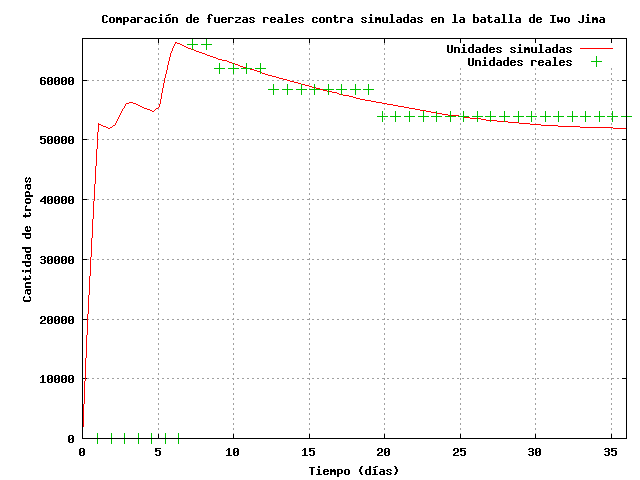
\includegraphics[width=12cm]{real_vs_sim.png}
\caption{\label{fig:realvssim}Comparación entre resultados reales y los simulados.}
\end{center}
\end{figure}

\newpage

\section{Haciendo historia}

¿Qué hubiese sucedido si la política de envío de refuerzos de Estados Unidos hubiese sido distinta?. En esta sección, analizamos como 
responde el sistema si variamos estas políticas, probando con distintas opciones y analizando los resultados.\\
Las dos políticas analizadas, que denominamos $g$ y $h$ son:

\begin{equation}
g(t) = \left\{ 
    \begin{array}{l l}
    \lfloor e^{2.5t} \rfloor + 2000 & \quad 0 \leq t \leq 4.6 \\
    0 & \quad t > 4.6\\
    \end{array} \right.
    \end{equation}

y

\begin{equation}
h(t) = \left\{ 
    \begin{array}{ll}
    54000 - \lfloor 9000t \rfloor & \quad 0 \leq t \leq 6 \\
    0 & \quad t > 6\\
    \end{array} \right.
    \end{equation}

Si observamos la gráfica presentada en la Figura \ref{fig:reinforce2} podemos ver que esta política resulta en un comportamiento del sistema
que equipara la cantidad de unidades de una y otra fuerza en cierto punto del tiempo $t$. Esto muestra que dicha planificación hubiese sido
menos conveniente que la que asumió EEUU en ese momento de la historia. Por otro lado, si vemos el comportamiento del sistema al elegir $h$
como política de refuerzos, presentado en la Figura \ref{fig:reinforce3}, podemos ver como la preponderancia de las tropas estadounidenses
aumenta y supera ampliamente a la japonesa de una manera mucho más conveniente que la elegida originalmente.

\begin{figure}[h]
\begin{center}
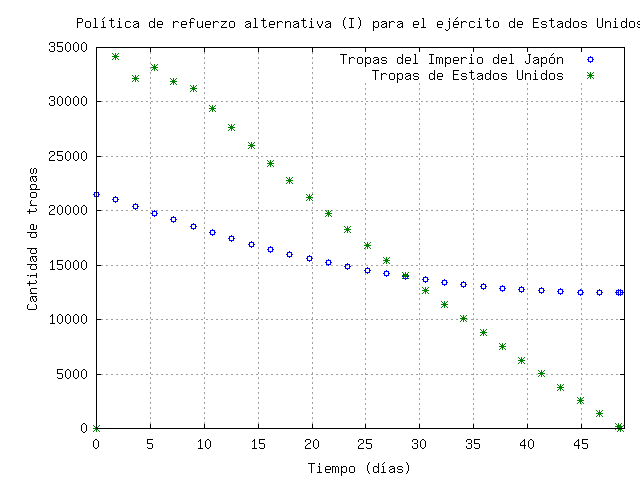
\includegraphics[width=12cm]{reinforce2.png}
\caption{\label{fig:reinforce2}Resultados del combate simulado usando la primer política de refuerzos alternativa.}
\end{center}
\end{figure}

\begin{figure}[h]
\begin{center}
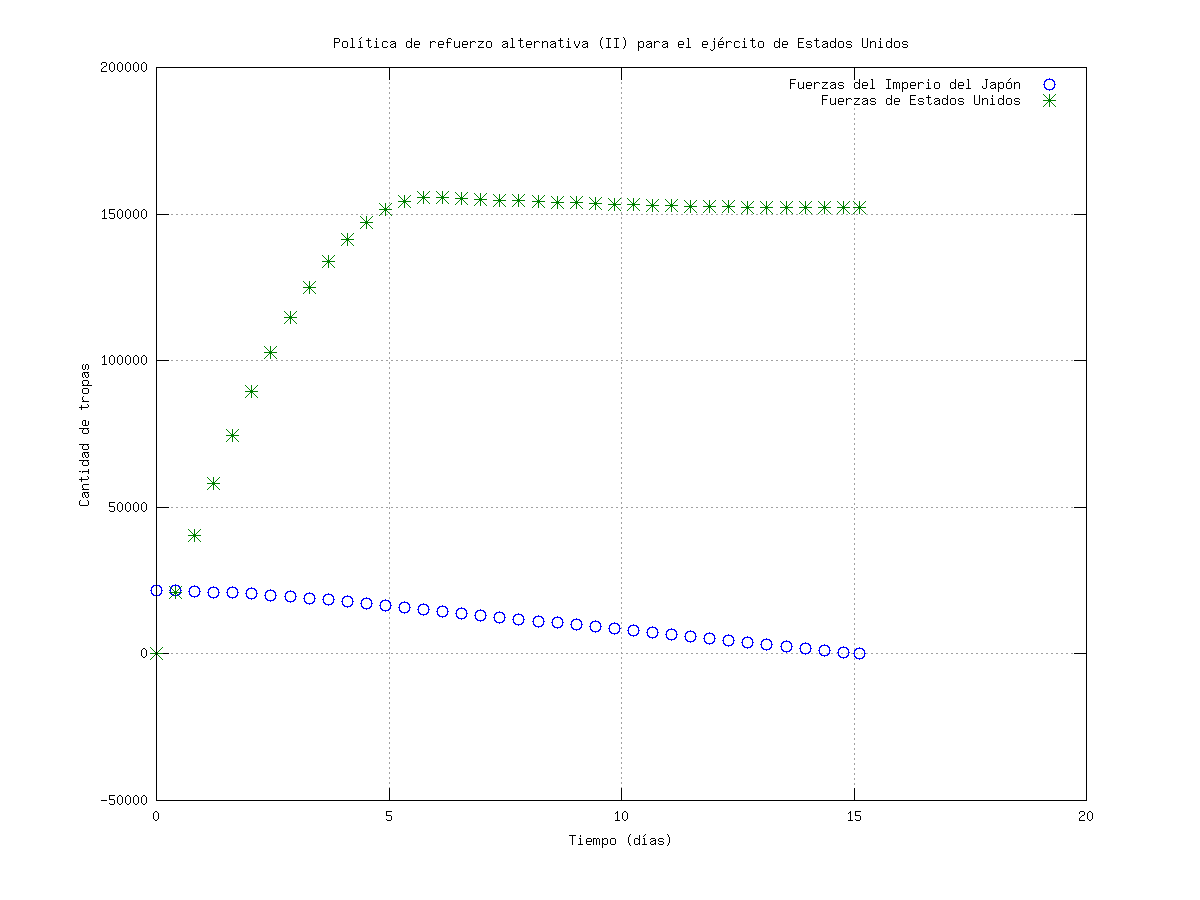
\includegraphics[width=12cm]{reinforce3.png}
\caption{\label{fig:reinforce3}Resultados del combate simulado usando la segunda política de refuerzos alternativa.}
\end{center}
\end{figure}



\section{Conclusiones}

La primera conclusión obtenida en este trabajo es que el modelo descripto en el mismo aproxima correctamente el comportamiento del sistema 
que se desea observar. Como conclusión a los cambios de política de refuerzos realizados, se puede decir que EEUU podría haber considerado una
mejor política de refuerzos, aunque requeriría un análisis socio-económico y político más profundo para poder determinar porque realmente no
lo hizo.\\
Puntos interesantes que se pueden observar de la primer simulación realizada, son los picos obtenidos al momento de la llegada de refuerzos
estadounidenses y las pérdidas iniciales durante la etapa de asentamiento, que se ven claramente en las irregularidades iniciales de la curva 
graficada.\\
Otra conclusión importante es la relación obtenida entre las fuerzas en combate. Particularmente, resaltar que ante una relación lineal de las
fuerzas, es decir, el caso en el que la constante $K$ es igual a $0$, la recta descripta nos proporciona bases de trabajo para estimar estadísticas
como la efectividad de las unidades militares de cada fuerza, contra las enemigas.





\end{document}
